\documentclass[aspectratio=169]{beamer}
\usepackage{tikz}
\usetikzlibrary{arrows.meta,positioning}
\begin{document}
\begin{frame}{Overlay states must each remain readable}
\centering
\begin{tikzpicture}[
  box/.style={draw, rounded corners, minimum width=34mm, minimum height=10mm},
  >=Latex
]
\node[box] (shock) at (-3,0) {Weather shock};
\only<1>{\node[box] (exposure) at (1,0) {Exposure};}
\only<2>{%
  \node[box] (exposure) at (1,0) {Exposure};
  \node[box] (mechanism) at (1.2,0) {Behavioral response};
}
\draw[->] (shock) -- node[above] {changes} (exposure);
\end{tikzpicture}
\end{frame}
\end{document}
